\subsection{Prose Backend}\label{sec:prose} %0.5p
\begin{figure}[t]
\centering
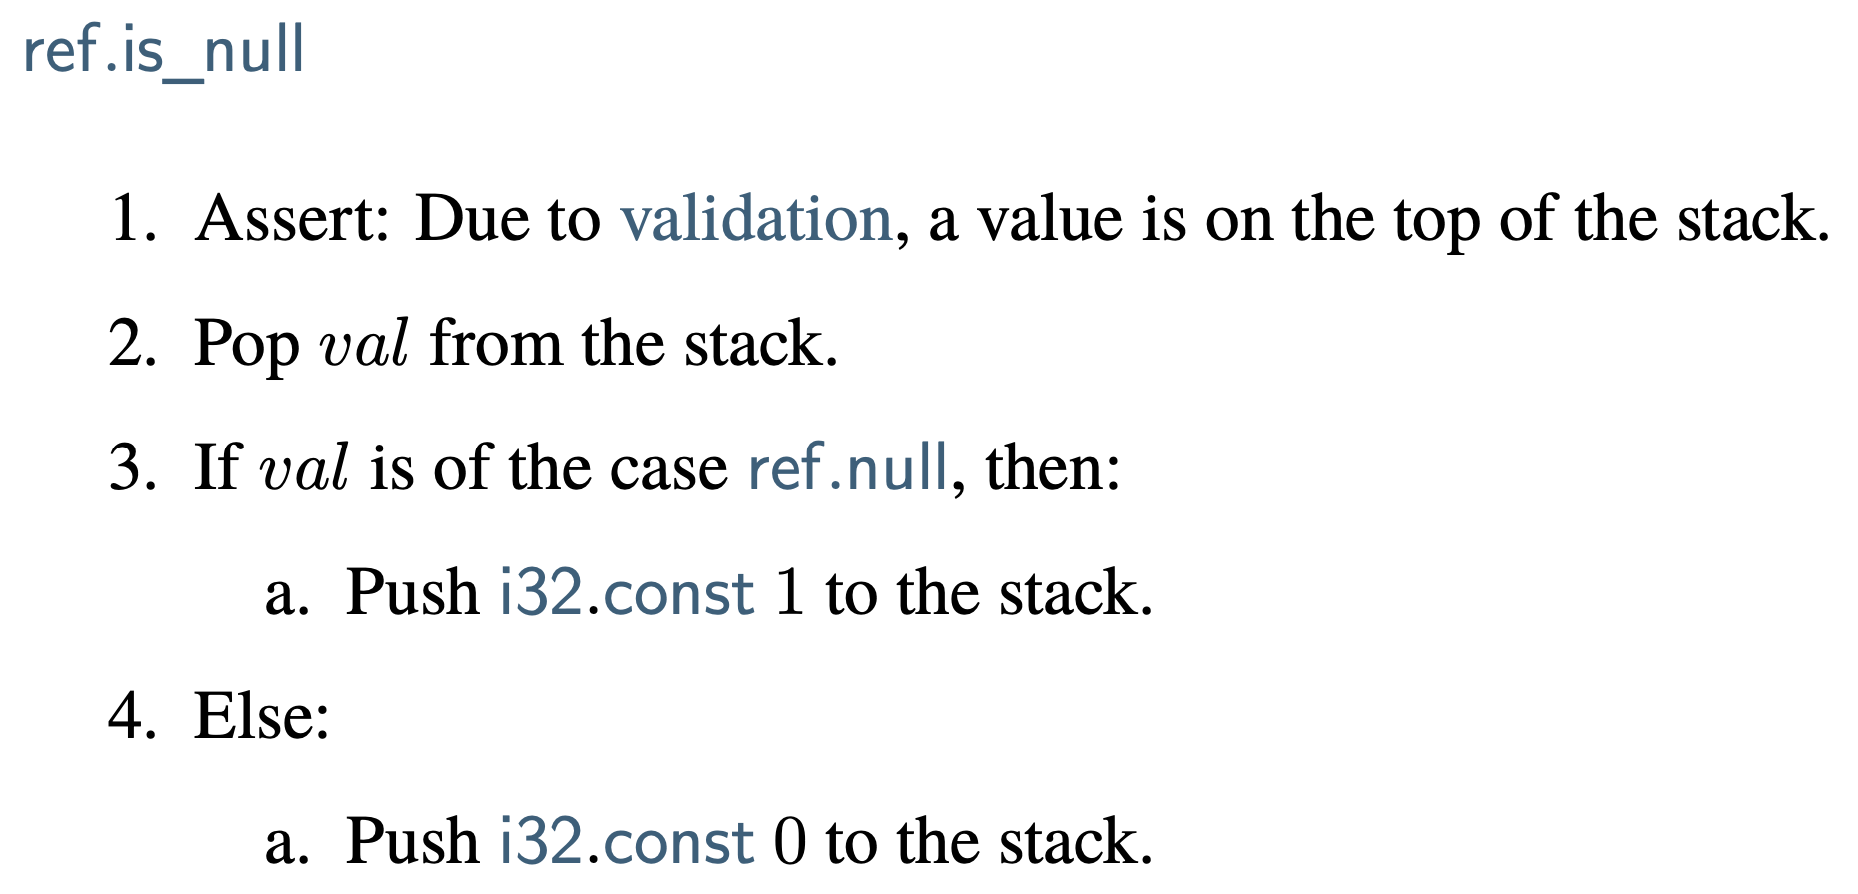
\includegraphics[width=.5\textwidth]{../img/genprose}
\vspace*{-1em}
\caption{Semantics of \inblue{\ensuremath{\mathsf{ref.is\_null}}} in a generated prose specification}
\label{fig:genprose}
\end{figure}

\al is designed to generate prose notation easily,
so the English prose specification can be generated directly from the semantics described in \al.
Fig.~\ref{fig:genprose} shows the prose pseudocode generated from the specification in Fig.~\ref{fig:dsl},
which is very close to the original handwritten prose description in Fig.~\ref{fig:spec1}.

\begin{itemize}
\item How to generate PDF with cross references
\item cf) error-prone generation of references done manually
\item systematic naming and bug detection?
\end{itemize}

Note that an \al expression may have a different prose rendering
depending on where it appears. For example, $|e|$ is rendered as 
``$|\expr|$'' or ``the length of $\expr$'' depending on whether it appears in
a mathematical context or not.
To support intuitive prose notation, some \al conditions are specially rendered.
For example, while ``$\kwnot$'' is rendered as ``not'' and ``$\kwisvalid\;\expr$''
is rendered as ``$\expr$ is valid,''
``$\kwnot \; (\kwisvalid \; \expr)$'' is rendered as ``$\expr$ is not valid''
rather than ``not $\expr$ is valid.''

